\section{Results}
\label{sec:results}

All numbers in this section come from the frozen confirmation (Qwen3-8B, held-out template, 384 histories
per task) unless marked otherwise.

\subsection{Competence}
\label{sec:results-competence}

\begin{table}[t]
\centering
\small
\setlength{\tabcolsep}{4pt}
\begin{tabular}{@{}lcccc@{}}
\toprule
Cell & Direct & No history & History & Competent \\
\midrule
routing seq.  & 0.988 & 0.953 & 0.858 & yes \\
routing int.  & 0.986 & 0.961 & 0.868 & yes \\
routing comp. & 0.982 & 0.953 & 0.846 & yes \\
\midrule
access seq.   & 0.916 & 0.867 & 0.831 & no \\
access int.   & 0.945 & 0.875 & 0.858 & no \\
access comp.  & 0.908 & 0.859 & 0.867 & no \\
\bottomrule
\end{tabular}
\caption{Strict accuracy on the confirmation data. \emph{Direct}: current state of the queried entity,
asked directly. \emph{No history}: decision on the current-only item. \emph{History}: decision over all
historical-construction items. Competent: direct $\ge 0.95$, no history $\ge 0.90$, invalid $\le 0.05$.
No answer was invalid.}
\label{tab:competence}
\end{table}

On the confirmation data, the routing cells meet all competence criteria and the access cells do not, mainly because current-only
decisions fall short of 0.90 (Table~\ref{tab:competence}). Asked for the \emph{initial} state on the
superseded items, the model answered correctly in 0.990 of routing and 0.973 of access cases. In routing,
then, the model reports the current state, reports the initial state, and applies the policy without
history at or above 0.95. Access results are reported below as fixed-grid averages over cells that do not
meet the competence criteria.

\subsection{Obsolete states change decisions}
\label{sec:results-h1}

\begin{figure*}[t]
\centering
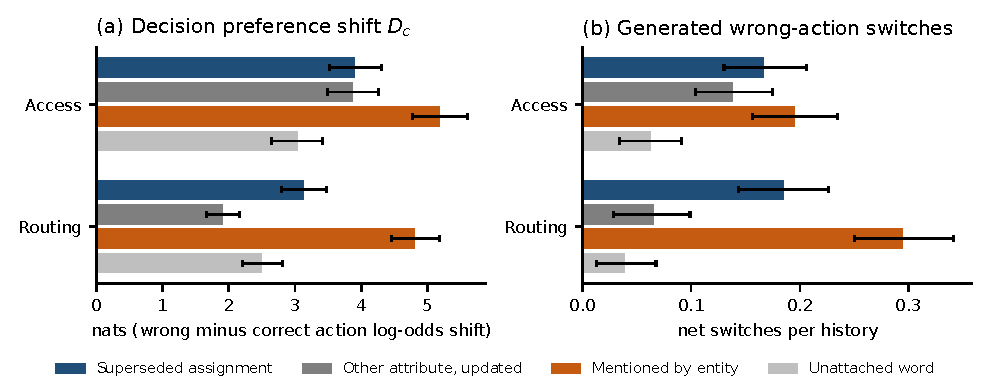
\includegraphics[width=\textwidth]{figures/constructions.pdf}
\caption{Decision effects by construction (confirmation, 384 histories per task, 95\% history-bootstrap
intervals). (a) $D_c$: increase in the wrong action's log-odds when the edited word implies the wrong
rather than the correct action. (b) Net switch rate toward the wrong action (mean over histories of $+1$,
$0$ or $-1$). Routing cells meet the competence criteria on the confirmation data; access cells do not.}
\label{fig:constructions}
\end{figure*}

H1 is supported in both tasks. In routing, when the superseded state implied the wrong action rather
than the correct one, the wrong action's log-odds rose by $D_{\mathrm{superseded}} = 3.133$ nats
(97.5\% interval $[2.743, 3.516]$). In access, where cells do not meet the competence criteria, the shift
was $3.904$ $[3.474, 4.346]$. For scale, editing the \emph{current} state itself, which legitimately
changes the correct action, moved the same quantity by $-8.197$ (routing) and $-10.100$ nats (access).

The shift reaches generated answers. In routing, the net switch rate toward the wrong action was $0.185$
$[0.143, 0.227]$: 75 histories switched to the wrong action and 4 to the correct one. In each routing
cell, it was between 0.164 and 0.227 (Table~\ref{tab:switch-cells}). In access it was $0.167$
$[0.130, 0.206]$ (65 against 1). Figure~\ref{fig:competence} shows the same effect as accuracy. In every
routing cell, decisions were correct in 0.906--0.953 of histories when the superseded state implied the
correct action, and in 0.727--0.750 when it implied the wrong one. The same records gave current- and
initial-state retrieval at or above 0.98.

\paragraph{Histories the model demonstrably tracks.} Aggregate retrieval accuracy does not show that the
switching histories are ones the model reads correctly. We therefore kept a history only if three
conditions held on the same records: the model retrieved the current state correctly under both members
of the pair, retrieved the initial state correctly under both superseded members, and decided the
current-only item correctly. This kept 348 of 384 routing histories for the superseded construction
(Table~\ref{tab:joint}). In them, the net switch rate toward the wrong action was $0.158$
$[0.118, 0.198]$: 58 histories switched to the wrong action and 3 to the correct one. The preference
shift was $2.990$ nats $[2.661, 3.342]$. Each routing cell keeps a net switch rate between 0.129 and
0.202. The effect is therefore not carried by histories in which the model misreads the record. In
access, the same restriction keeps 284 of 384 histories and gives a net switch rate of $0.176$
$[0.134, 0.218]$ (50 against 0).

\begin{table}[t]
\centering
\small
\setlength{\tabcolsep}{3pt}
\resizebox{\columnwidth}{!}{%
\begin{tabular}{@{}lcccc@{}}
\toprule
& Kept & $D_{\mathrm{superseded}}$ & Net switch rate & Switched \\
\midrule
routing seq.  & 118/128 & 2.959 & 0.144 $[0.076, 0.220]$ & 19 / 2 \\
routing int.  & 114/128 & 3.252 & 0.202 $[0.132, 0.281]$ & 24 / 1 \\
routing comp. & 116/128 & 2.764 & 0.129 $[0.069, 0.190]$ & 15 / 0 \\
routing, all  & 348/384 & 2.990 & 0.158 $[0.118, 0.198]$ & 58 / 3 \\
\midrule
access, all   & 284/384 & 4.059 & 0.176 $[0.134, 0.218]$ & 50 / 0 \\
\bottomrule
\end{tabular}}
\caption{Superseded construction, restricted to histories with correct current-state retrieval under both
members, correct initial-state retrieval under both members, and a correct current-only decision. Kept:
histories retained out of those in the cell. Switched: histories switched to the wrong / to the correct
action. 95\% history-bootstrap intervals. Retained sets differ slightly across constructions because
condition (i) is checked per construction. Condition (ii) is checked on the history's superseded members for
every construction, because the initial-state query is asked only there.}
\label{tab:joint}
\end{table}

\begin{figure*}[t]
\centering
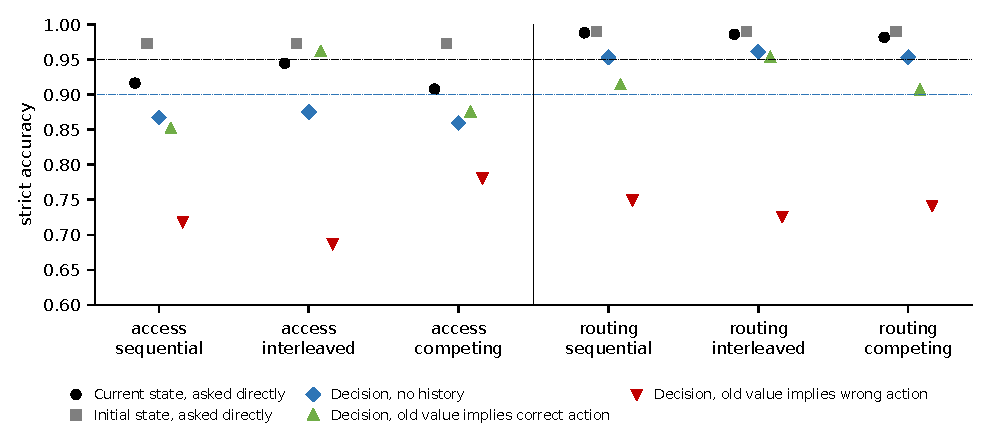
\includegraphics[width=\textwidth]{figures/competence.pdf}
\caption{Retrieval and decision accuracy on the same confirmation records, per cell. Initial-state
retrieval is reported per task. Routing (left) meets the competence criteria on the confirmation data; access (right) does not.}
\label{fig:competence}
\end{figure*}

\subsection{Supersession adds pressure; a mention adds comparable pressure}
\label{sec:results-h2}

This section reports Qwen3-8B, where a mention adds more pressure than a superseded assignment;
\S\ref{sec:results-replication} shows that in Qwen3-14B it adds comparable pressure. H2 compares the
superseded assignment with an assignment of the same word to a different attribute that was later updated. It is supported in routing, $\Delta_{\mathrm{semantic}} = +1.224$ $[0.973, 1.485]$, with
generated switches agreeing ($+0.120$ $[0.076, 0.164]$). In routing, then, the attribute that was
superseded matters. In access (non-competent cells) the contrast is inconclusive: $+0.035$
$[-0.318, 0.400]$, switches $+0.029$ $[-0.016, 0.073]$.

The mention control, a secondary outcome, shows that supersession is not the largest source of pressure
in Qwen3-8B.
When the same entity only \emph{mentioned} the word, the effect was larger than for the superseded
assignment. In routing, $D_{\mathrm{entity\,mention}} = 4.807$ against $3.133$, so
$\Delta_{\mathrm{mention}} = -1.675$ $[-1.896, -1.441]$. Net switches were $0.294$ (113 to wrong, 0 to
correct) against $0.185$, difference $-0.109$ $[-0.156, -0.065]$. In access, $5.182$ against $3.904$
($\Delta_{\mathrm{mention}} = -1.278$ $[-1.579, -0.977]$). Switches there were $0.195$ (76 against 1)
against $0.167$, an inconclusive difference. A word attached to no entity still shifted preference
substantially, by $2.496$ (routing) and $3.043$ nats (access), but rarely changed a generated decision
($0.039$ and $0.062$). Score shifts of similar size can thus have very different behavioral
consequences. The ordering holds in the restricted routing histories of Table~\ref{tab:joint}. Net switch
rates there are $0.278$ for the mention, $0.158$ for the superseded assignment, $0.048$ for the updated
unrelated attribute and $0.034$ for the unattached word.

Across four earlier, non-confirmatory splits, $\Delta_{\mathrm{mention}}$ never favored the superseded
assignment, but its size varied with the template (Appendix~\ref{app:tables}, Figure~\ref{fig:replication}).

\subsection{Easy-query sensitivity adds nothing to failure prediction}
\label{sec:results-h3}



The edit strongly affected easy retrieval scores: the mean $R_{\mathrm{easy}}$ on superseded items was
$8.096$ nats in access and $10.878$ in routing. That sensitivity added nothing beyond the pre-decision
features under the specified logistic model (Table~\ref{tab:h3} in Appendix~\ref{app:tables}). Pre-decision features reduced log loss from $0.414$ to
$0.346$ and reached AUROC $0.780$. Adding $R_{\mathrm{easy}}$ changed log loss by $+0.0004$ nats,
interval $[-0.0011, 0.0019]$; the upper end is under 3\% of what the simple features already gain. The
result is the same in each task and for the wrong-answer outcome. It replicates in Qwen3-14B: AUROC
$0.684$ without and $0.685$ with $R_{\mathrm{easy}}$, log-loss gain $-0.0001$ $[-0.0027, 0.0022]$. Within
this design,
$R_{\mathrm{easy}}$ describes how retrieval scores respond to the edit; it does not diagnose decision
vulnerability.

\subsection{Replication in Qwen3-14B, and a model that was not eligible}
\label{sec:results-replication}
\label{sec:results-gemma}

\begin{table*}[t]
\centering
\small
\setlength{\tabcolsep}{4pt}
\resizebox{\textwidth}{!}{%
\begin{tabular}{@{}llccccc@{}}
\toprule
Model & Task (competent cells) & $n$ & $D_{\mathrm{superseded}}$ & $\Delta_{\mathrm{semantic}}$ & $\Delta_{\mathrm{mention}}$ & Net switch rate \\
\midrule
Qwen3-8B & routing (comp., int., seq.) & 384 & $+3.133$ {\scriptsize $[+2.743, +3.516]$} & $+1.224$ {\scriptsize $[+0.973, +1.485]$} & $-1.675$ {\scriptsize $[-1.896, -1.441]$} & $+0.185$ {\scriptsize $[+0.143, +0.227]$} \\
Qwen3-8B & access & \multicolumn{5}{l}{no competent cell} \\
\midrule
Qwen3-14B & routing (comp., int., seq.) & 384 & $+4.785$ {\scriptsize $[+4.244, +5.354]$} & $+0.866$ {\scriptsize $[+0.417, +1.328]$} & $+0.248$ {\scriptsize $[-0.117, +0.601]$} & $+0.167$ {\scriptsize $[+0.130, +0.206]$} \\
Qwen3-14B & access & \multicolumn{5}{l}{no competent cell} \\
\midrule
Gemma 3 4B & \multicolumn{6}{l}{not eligible: no competent cell at the gate} \\
\bottomrule
\end{tabular}}
\caption{Confirmation results per model, on the task-cells that met the competence criteria \emph{on the confirmation data} (the rule used in the text and in Table~\ref{tab:competence}). $D$ and $\Delta$ in nats; $D_{\mathrm{superseded}}$ and $\Delta_{\mathrm{semantic}}$ with 97.5\% intervals, $\Delta_{\mathrm{mention}}$ and the superseded net switch rate with 95\% intervals (history bootstrap). Models are reported separately, never pooled. The replication amendment defined competent cells by each model\textquoteright s frozen gate (Table~\ref{tab:models-gate}); gate-rule estimates are in Appendix~\ref{app:tables}.}
\label{tab:cross-model}
\end{table*}


Qwen3-14B was added under an amendment dated before any of its data were scored, with the same rows, rules
and runtime (Appendix~\ref{app:history}). Its frozen gate passed in all three routing cells and in no access
cell (Table~\ref{tab:models-gate}). On the confirmation, routing retrieval was 0.989--0.997 for the current
state and 0.997 for the initial state. Current-only decisions were 0.977--0.992 correct.

Table~\ref{tab:cross-model} compares the two models on the cells competent on the confirmation data. The obsolete-state effect
replicates. In routing, $D_{\mathrm{superseded}} = 4.785$ nats and the net switch rate is $0.167$ (67
histories switched to wrong, 3 to correct). In the routing histories Qwen3-14B demonstrably tracks (376 of
384), it is $0.165$ $[0.128, 0.205]$ (Table~\ref{tab:joint-by-model}). Supersession again adds preference
over an updated unrelated attribute: $\Delta_{\mathrm{semantic}} = +0.866$ $[0.417, 1.328]$ in routing.
In generated switches, however, the two constructions are close in this model ($0.167$ against $0.146$).
The mention result differs from Qwen3-8B. In Qwen3-14B the mention moves routing decisions as much as the
superseded assignment does: net switch rates are $0.169$ against $0.167$ over all routing histories, and
$0.168$ against $0.165$ in the tracked histories (Table~\ref{tab:joint-by-model}), with
$\Delta_{\mathrm{mention}} = +0.248$ $[-0.117, 0.601]$, an inconclusive difference. In access
(non-competent cells) the superseded assignment moved preference more than the mention
($\Delta_{\mathrm{mention}} = +0.845$ $[0.425, 1.255]$). In both models, then, an incidental mention
produces interference of the same order as a superseded assignment. Whether it exceeds it is
model-specific.

Gemma 3 4B was added under a model list frozen before any of its data were scored. On the gate split, no
cell met the criteria: current-only decision accuracy was 0.609--0.719, direct retrieval 0.916--0.964
(Table~\ref{tab:models-gate}), while initial-state retrieval in development was 0.984. Gemma reads these
records but does not apply the policy reliably, so no confirmation split was generated for it. This is an
eligibility result, not evidence for or against stale-state interference in Gemma.
